\chapter{Least Squares}

\section{An Example: Measurement Problem}

\begin{problem}
    已知测量量路段长度: $ A D=89, A C=67, B D=53, A B=35, C D=20 $ $ , x_{1}, x_{2} $ 和 $ x_{3} $ 的长度是多少?
\end{problem}

\begin{FigureCenter}{Measurement Problem}
    

\tikzset{every picture/.style={line width=0.75pt}} %set default line width to 0.75pt        

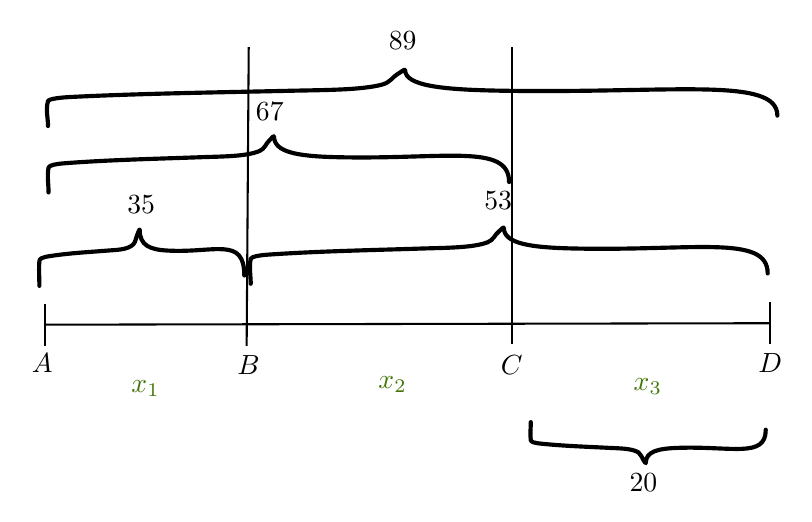
\begin{tikzpicture}[x=0.75pt,y=0.75pt,yscale=-1,xscale=1]
%uncomment if require: \path (0,300); %set diagram left start at 0, and has height of 300

%Straight Lines [id:da18809251009182648] 
\draw    (100,143) -- (449,142.29) ;
%Straight Lines [id:da4295294079118699] 
\draw    (100,132.85) -- (100,153.15) ;
%Straight Lines [id:da08559662247482214] 
\draw    (198,9.29) -- (197,153.15) ;
%Straight Lines [id:da8061715298122138] 
\draw    (325,9.29) -- (325,152.15) ;
%Straight Lines [id:da1891846903803609] 
\draw    (449,132.15) -- (449,152.44) ;
%Shape: Free Drawing [id:dp5156036617765727] 
\draw  [color={rgb, 255:red, 0; green, 0; blue, 0 }  ][line width=1.5] [line join = round][line cap = round] (101.3,47.29) .. controls (101.3,43.29) and (100.09,39.28) .. (101.3,35.29) .. controls (101.67,34.1) and (107.95,33.51) .. (112.28,33.29) .. controls (146.53,31.59) and (183.69,31.09) .. (218.43,30.29) .. controls (233.89,29.94) and (252.54,29.98) .. (262.36,27.29) .. controls (266.42,26.18) and (267.24,23.63) .. (269.68,22.29) .. controls (270.9,21.63) and (273.34,19.55) .. (273.34,20.29) .. controls (273.34,27.91) and (291.11,29.83) .. (320.92,30.29) .. controls (402.67,31.57) and (452.7,23.35) .. (452.7,42.29) ;
%Shape: Free Drawing [id:dp895862543035038] 
\draw  [color={rgb, 255:red, 0; green, 0; blue, 0 }  ][line width=1.5] [line join = round][line cap = round] (101.56,79.29) .. controls (101.56,75.29) and (100.79,71.28) .. (101.56,67.29) .. controls (101.79,66.1) and (105.76,65.51) .. (108.49,65.29) .. controls (130.11,63.59) and (153.58,63.09) .. (175.52,62.29) .. controls (185.28,61.94) and (197.06,61.98) .. (203.25,59.29) .. controls (205.82,58.18) and (206.34,55.63) .. (207.88,54.29) .. controls (208.65,53.63) and (210.19,51.55) .. (210.19,52.29) .. controls (210.19,59.91) and (221.41,61.83) .. (240.24,62.29) .. controls (291.85,63.57) and (323.44,55.35) .. (323.44,74.29) ;
%Shape: Free Drawing [id:dp019817472694717342] 
\draw  [color={rgb, 255:red, 0; green, 0; blue, 0 }  ][line width=1.5] [line join = round][line cap = round] (198.97,123.29) .. controls (198.97,119.29) and (198.11,115.28) .. (198.97,111.29) .. controls (199.23,110.1) and (203.69,109.51) .. (206.75,109.29) .. controls (231.03,107.59) and (257.37,107.09) .. (281.99,106.29) .. controls (292.94,105.94) and (306.17,105.98) .. (313.12,103.29) .. controls (316,102.18) and (316.58,99.63) .. (318.31,98.29) .. controls (319.18,97.63) and (320.91,95.55) .. (320.91,96.29) .. controls (320.91,103.91) and (333.5,105.83) .. (354.63,106.29) .. controls (412.57,107.57) and (448.03,99.35) .. (448.03,118.29) ;
%Shape: Free Drawing [id:dp36042969413065307] 
\draw  [color={rgb, 255:red, 0; green, 0; blue, 0 }  ][line width=1.5] [line join = round][line cap = round] (97.14,124.29) .. controls (97.14,120.29) and (96.8,116.28) .. (97.14,112.29) .. controls (97.24,111.1) and (99.01,110.51) .. (100.23,110.29) .. controls (109.85,108.59) and (120.29,108.09) .. (130.05,107.29) .. controls (134.39,106.94) and (139.63,106.98) .. (142.39,104.29) .. controls (143.53,103.18) and (143.76,100.63) .. (144.44,99.29) .. controls (144.79,98.63) and (145.47,96.55) .. (145.47,97.29) .. controls (145.47,104.91) and (150.46,106.83) .. (158.84,107.29) .. controls (181.8,108.57) and (195.86,100.35) .. (195.86,119.29) ;
%Shape: Free Drawing [id:dp5719345430074279] 
\draw  [color={rgb, 255:red, 0; green, 0; blue, 0 }  ][line width=1.5] [line join = round][line cap = round] (333.9,189.94) .. controls (333.9,192.86) and (333.5,195.79) .. (333.9,198.7) .. controls (334.01,199.57) and (336.04,200) .. (337.43,200.16) .. controls (348.47,201.4) and (360.44,201.77) .. (371.63,202.35) .. controls (376.61,202.6) and (382.62,202.58) .. (385.78,204.54) .. controls (387.09,205.35) and (387.35,207.21) .. (388.14,208.19) .. controls (388.53,208.67) and (389.32,210.19) .. (389.32,209.65) .. controls (389.32,204.09) and (395.05,202.69) .. (404.65,202.35) .. controls (430.99,201.42) and (447.1,207.42) .. (447.1,193.59) ;

% Text Node
\draw (92,155.4) node [anchor=north west][inner sep=0.75pt]    {$A$};
% Text Node
\draw (191,156.4) node [anchor=north west][inner sep=0.75pt]    {$B$};
% Text Node
\draw (318,156.4) node [anchor=north west][inner sep=0.75pt]    {$C$};
% Text Node
\draw (442,155.4) node [anchor=north west][inner sep=0.75pt]    {$D$};
% Text Node
\draw (140,168.4) node [anchor=north west][inner sep=0.75pt]  [color={rgb, 255:red, 65; green, 117; blue, 5 }  ,opacity=1 ]  {$x_{1}$};
% Text Node
\draw (259,166.4) node [anchor=north west][inner sep=0.75pt]  [color={rgb, 255:red, 65; green, 117; blue, 5 }  ,opacity=1 ]  {$x_{2}$};
% Text Node
\draw (382,167.4) node [anchor=north west][inner sep=0.75pt]  [color={rgb, 255:red, 65; green, 117; blue, 5 }  ,opacity=1 ]  {$x_{3}$};
% Text Node
\draw (264,0.4) node [anchor=north west][inner sep=0.75pt]    {$89$};
% Text Node
\draw (200,34.4) node [anchor=north west][inner sep=0.75pt]    {$67$};
% Text Node
\draw (310,77.4) node [anchor=north west][inner sep=0.75pt]    {$53$};
% Text Node
\draw (138,79.4) node [anchor=north west][inner sep=0.75pt]    {$35$};
% Text Node
\draw (380,213.4) node [anchor=north west][inner sep=0.75pt]    {$20$};


\end{tikzpicture}
\end{FigureCenter}

由 $ x_{1}, x_{2} $ 和 $ x_{3} $ 的关系可得方程组:
\begin{equation}
\left\{\begin{array}{r}
x_{1}+x_{2}+x_{3}=89 \\
x_{1}+x_{2}=67 \\
x_{2}+x_{3}=53 \\
x_{1}=35 \\
x_{3}=20
\end{array} \Leftrightarrow A x=b, A=\left[\begin{array}{lll}
1 & 1 & 1 \\
1 & 1 & 0 \\
0 & 1 & 1 \\
1 & 0 & 0 \\
0 & 0 & 1
\end{array}\right], b=\left[\begin{array}{l}
89 \\
67 \\
53 \\
35 \\
20
\end{array}\right]\right.
\end{equation}

取后三个式子求解方程组,回代前两个式子

\begin{equation}\displaystyle  \begin{array}{{>{\displaystyle}l}}
\left\{\begin{array}{ r }
x_{2} +x_{3} =53\\
x_{1} =35\\
x_{3} =20
\end{array} \Rightarrow x_{1} =35,x_{2} =33,x_{3} =20.\right. \\
\left\{\begin{array}{ r }
x_{1} +x_{2} +x_{3} =88\neq 89\\
x_{1} +x_{2} =68\neq 67
\end{array}\right. 
\end{array}\end{equation}
     

由于测量存在误差,方程组之间相互矛盾,该超定方程组无解。

\section{最小二乘问题}

\begin{problem}[最小二乘问题]
    寻找该方程组的近似解,并尽可能逼近方程组的目标$b$, 即残差向量 $ r=A x-b $ 某种度量下尽可能小

    \begin{equation} \min _{x}\|A x-b\|_{2}^{2}=\|r\|_{2}^{2} \quad (\ell_2范数度量残差) \end{equation}
\end{problem}


使用$\ell_1$、$\ell_\infty$等也可以度量误差,但是函数在零点处不光滑,不能求导。

\begin{problem}[求解最小二乘解]
    给定 $ {A} \in \mathbb{R}^{m \times n}, {~b} \in \mathbb{R}^{m} $, 求解 $ x \in \mathbb{R}^{n} $ 让目标函数最小

\begin{equation} \min _{x}\|A x-b\|_{2}^{2}=\min _{x} \sum_{i=1}^{m}\left(\sum_{j=1}^{n} A_{i j} x_{j}-b_{i}\right)^{2} \end{equation}
\end{problem}

\begin{notation}[最小二乘法的解]
    记最小二乘法的解为 $ \hat{x} $

    \begin{equation}
    \hat{x}=\arg \underset{x}{\min}\|A x-b\|_{2}^{2}=\arg \underset{x}{\min} \sum_{i=1}^{m}\left(\sum_{j=1}^{n} A_{i j} x_{j}-b_{i}\right)^{2}
    \end{equation}
\end{notation}

\begin{example}
    \begin{equation} f(x)=\|A x-b\|_{2}^{2}, {A}=\left[\begin{array}{cc}2 & 0 \\ -1 & 1 \\ 0 & 2\end{array}\right], b=\left[\begin{array}{c}1 \\ 0 \\ -1\end{array}\right] \end{equation}

    求解\begin{equation}\hat{x} = \arg \underset{x}{\min} \|A x-b\|_{2}^{2}\end{equation}

    解:
    \begin{equation} f(x)=\|A x-b\|_{2}^{2}=\left(2 x_{1}-1\right)^{2}+\left(-x_{1}+x_{2}\right)^{2}+\left(2 x_{2}+1\right)^{2} \end{equation}

    \begin{equation} \frac{\partial f}{\partial x_{1}}=10 x_{1}-2 x_{2}-4 , \frac{\partial f}{\partial x_{2}}=-2 x_{1}+10 x_{2}+4 \end{equation}

    \begin{equation} \nabla f(x)=\left[\begin{array}{l}\dfrac{\partial f}{\partial x_{1}} \\ \dfrac{\partial f}{\partial x_{2}}\end{array}\right]=0 \Rightarrow \hat{x}=\left(\frac{1}{3},-\frac{1}{3}\right)^{T} \end{equation}
\end{example}


\begin{theorem}
    设最小二乘法的解为 $ \hat{x} $ ,满足:
    \begin{equation}
    \|A \hat{x}-b\|_{2}^{2} \leq\|A x-b\|_{2}^{2}, \forall x \in \mathbf{R}^{n}
    \end{equation}

    当残差 $ \hat{r}=A \hat{x}-b=0 $ 时,则 $ \hat{x} $ 是线性方程组 $ A x=b $ 的解; 否则其为误差最小平方和意义下方程组的近似解。
\end{theorem}



\section{求解最小二乘法}

给定 $ A \in \mathbb{R}^{m \times n}, b \in \mathbb{R}^{m}, x \in \mathbb{R}^{n} $ 目标函数:
\begin{equation}
f(x)=\|A x-b\|_{2}^{2}=\sum_{i=1}^{m}\left(\sum_{j=1}^{n} A_{i j} x_{j}-b_{i}\right)^{2}
\end{equation}

为使目标函数最小,求最优解 $ \hat{x}:\hat{x}=\arg \underset{x}{\min} f(x) $

\begin{theorem}
    可微函数 $ f(x) $ 的最优解 $ \hat{x} $ 满足条件:梯度 $ \nabla f(\hat{x})=\mathbf{0} $ , 即:
\begin{equation}
\nabla f(\hat{x})=\left[\begin{array}{c}
\dfrac{\partial f}{\partial x_{1}}(\hat{x}) \\
\vdots \\
\dfrac{\partial f}{\partial x_{n}}(\hat{x})
\end{array}\right]=2 A^{T}(A \hat{x}-b)=0
\end{equation}
\end{theorem}

\begin{theorem}[正规方程与最小二乘解]
    \begin{equation} A^{T} A x=A^{T} b \end{equation}

    $A$的列向量\textbf{线性无关}时,则 $ \hat{x}=\left(A^{T} A\right)^{-1} A^{T} b $. 
\end{theorem}

\begin{proof}
    设函数 $ g_{i}(x)=\sum_{j=1}^{n} A_{i j} x_{j}-b_{i} $ ,则有

    
        \begin{equation}g_{i}( x) =\sum\limits _{j=1}^{n} A_{ij} x_{j} -b_{i} \Rightarrow \left(\begin{array}{ c c c c c }
        A_{1,1} & \cdots  & A_{1,k} & \cdots  & A_{1,n}\\
        \vdots  &  & \vdots  &  & \vdots \\
        \boldsymbol{\textcolor[rgb]{0.72,0.33,0.31}{A}\textcolor[rgb]{0.72,0.33,0.31}{_{j,1}}} & \boldsymbol{\textcolor[rgb]{0.72,0.33,0.31}{\cdots }} & \boldsymbol{\textcolor[rgb]{0.72,0.33,0.31}{A}\textcolor[rgb]{0.72,0.33,0.31}{_{j,k}}} & \boldsymbol{\textcolor[rgb]{0.72,0.33,0.31}{\cdots }} & \boldsymbol{\textcolor[rgb]{0.72,0.33,0.31}{A}\textcolor[rgb]{0.72,0.33,0.31}{_{j,n}}}\\
        \vdots  &  & \vdots  &  & \vdots \\
        A_{m,1} & \cdots  & A_{m,k} & \cdots  & A_{m,n}
        \end{array}\right)\left(\begin{array}{ c }
        \boldsymbol{\textcolor[rgb]{0.72,0.33,0.31}{x}\textcolor[rgb]{0.72,0.33,0.31}{_{1}}}\\
        \boldsymbol{\textcolor[rgb]{0.72,0.33,0.31}{\vdots }}\\
        \boldsymbol{\textcolor[rgb]{0.72,0.33,0.31}{x}\textcolor[rgb]{0.72,0.33,0.31}{_{j}}}\\
        \boldsymbol{\textcolor[rgb]{0.72,0.33,0.31}{\vdots }}\\
        \boldsymbol{\textcolor[rgb]{0.72,0.33,0.31}{x}\textcolor[rgb]{0.72,0.33,0.31}{_{n}}}
        \end{array}\right) -\left(\begin{array}{ c }
        \textcolor[rgb]{0,0,0}{b_{1}}\\
        \textcolor[rgb]{0,0,0}{\vdots }\\
        \textcolor[rgb]{0.72,0.33,0.31}{b\boldsymbol{_{j}}}\\
        \textcolor[rgb]{0,0,0}{\vdots }\\
        \textcolor[rgb]{0,0,0}{b_{n}}
        \end{array}\right)\end{equation}
    
    所以
    \begin{equation}\begin{aligned} 
        f(x)&=\|A x-b\|_{2}^{2}
        &=\sum_{i=1}^{m}\left(\sum_{j=1}^{n} A_{i j} x_{j}-b_{i}\right)^{2}
        &=\sum_{i=1}^{m}\left(g_{i}(x)\right)^{2} 
    \end{aligned}\end{equation}

    函数 $ f(x) $ 对变量 $ x_{k} $ 偏导为
    
    \begin{equation} \frac{\partial f(x)}{\partial x_{k}}=\sum_{i=1}^{m}\left(\left(2 g_{i}(x)\right)\left(\frac{\partial g_{i}(x)}{\partial x_{k}}\right)\right) \end{equation}


    又因为
    \begin{equation} \frac{\partial g_{i}(x)}{\partial x_{k}}=A_{i k} \end{equation}


    所以
    \begin{equation} \begin{aligned} 
        \frac{\partial f}{\partial x_{k}}(x) 
        &=\sum_{i=1}^{m} 2\left(g_{i}(x)\right)\left(A_{i k}\right) \\
        &=2 \sum_{i=1}^{m}\left(\left(\sum_{j=1}^{n} A_{i j} x_{j}-b_{i}\right)\left(A_{i k}\right)\right) 
        \\ &=2 \sum_{i=1}^{m}\left(\left(\sum_{j=1}^{n} A_{i j} x_{j}\right)\left(A_{i k}\right)\right)-2 \sum_{i=1}^{m}\left(\left(b_{i}\right)\left(A_{i k}\right)\right) \end{aligned} \end{equation}

    注意有
        

    \begin{equation}\sum\limits _{j=1}^{n} A_{ij} x_{j} =\left(\begin{array}{ c c c c c }
    A_{1,1} & \cdots  & A_{1,k} & \cdots  & A_{1,n}\\
    \vdots  &  & \vdots  &  & \vdots \\
    \boldsymbol{\textcolor[rgb]{0.72,0.33,0.31}{A}\textcolor[rgb]{0.72,0.33,0.31}{_{j,1}}} & \boldsymbol{\textcolor[rgb]{0.72,0.33,0.31}{\cdots }} & \boldsymbol{\textcolor[rgb]{0.72,0.33,0.31}{A}\textcolor[rgb]{0.72,0.33,0.31}{_{j,k}}} & \boldsymbol{\textcolor[rgb]{0.72,0.33,0.31}{\cdots }} & \boldsymbol{\textcolor[rgb]{0.72,0.33,0.31}{A}\textcolor[rgb]{0.72,0.33,0.31}{_{j,n}}}\\
    \vdots  &  & \vdots  &  & \vdots \\
    A_{m,1} & \cdots  & A_{m,k} & \cdots  & A_{m,n}
    \end{array}\right)\left(\begin{array}{ c }
    \boldsymbol{\textcolor[rgb]{0.72,0.33,0.31}{x}\textcolor[rgb]{0.72,0.33,0.31}{_{1}}}\\
    \boldsymbol{\textcolor[rgb]{0.72,0.33,0.31}{\vdots }}\\
    \boldsymbol{\textcolor[rgb]{0.72,0.33,0.31}{x}\textcolor[rgb]{0.72,0.33,0.31}{_{j}}}\\
    \boldsymbol{\textcolor[rgb]{0.72,0.33,0.31}{\vdots }}\\
    \boldsymbol{\textcolor[rgb]{0.72,0.33,0.31}{x}\textcolor[rgb]{0.72,0.33,0.31}{_{n}}}
    \end{array}\right) =\left(\begin{array}{ c }
    Result_{1}\\
    \vdots \\
    \boldsymbol{\textcolor[rgb]{0.72,0.33,0.31}{Result}\textcolor[rgb]{0.72,0.33,0.31}{_{k}}}\\
    \vdots \\
    Result_{m}
    \end{array}\right) =Ax\end{equation}

    \begin{equation}\displaystyle \sum _{i=1}^{m}\left(\underbrace{\left(\sum _{j=1}^{n} A_{ij} x_{j}\right)}_{Result}( A_{ik})\right) =\begin{array}{ c }
    A_{1,\textcolor[rgb]{0.29,0.56,0.89}{\boldsymbol{k}}} \times Result_{1}\\
    +\\
    \vdots \\
    +\\
    \boldsymbol{\textcolor[rgb]{0.72,0.33,0.31}{A_{i,\textcolor[rgb]{0.29,0.56,0.89}{\boldsymbol{k}}} \times Result}\textcolor[rgb]{0.72,0.33,0.31}{_{i}}}\\
    +\\
    \vdots \\
    +\\
    A\textcolor[rgb]{0.29,0.56,0.89}{\boldsymbol{_{\textcolor[rgb]{0,0,0}{m,} k}}} \times Result_{m}
    \end{array} =\left(\begin{array}{ c }
    A_{1,\textcolor[rgb]{0.29,0.56,0.89}{\boldsymbol{k}}}\\
    \vdots \\
    A_{i,\textcolor[rgb]{0.29,0.56,0.89}{\boldsymbol{k}}}\\
    \vdots \\
    A_{m,\textcolor[rgb]{0.29,0.56,0.89}{\boldsymbol{k}}}
    \end{array}\right)^{T} Ax=a_{\textcolor[rgb]{0.29,0.56,0.89}{\boldsymbol{k}}}^{T} Ax\end{equation}
        
    类似地,有 
    
    \begin{equation}\displaystyle \sum _{i=1}^{m}(( b_{i})( A_{ik})) =\begin{array}{ c }
    A_{1,\textcolor[rgb]{0.29,0.56,0.89}{\boldsymbol{k}}} \times b_{1}\\
    +\\
    \vdots \\
    +\\
    \boldsymbol{\textcolor[rgb]{0.72,0.33,0.31}{A}\textcolor[rgb]{0.72,0.33,0.31}{_{i,\textcolor[rgb]{0.29,0.56,0.89}{\boldsymbol{k}}}}\textcolor[rgb]{0.72,0.33,0.31}{\times b}\textcolor[rgb]{0.72,0.33,0.31}{_{i}}}\\
    +\\
    \vdots \\
    +\\
    A\textcolor[rgb]{0.29,0.56,0.89}{\boldsymbol{_{\textcolor[rgb]{0,0,0}{m,} k}}} \times b_{m}
    \end{array} =a_{\textcolor[rgb]{0.29,0.56,0.89}{\boldsymbol{k}}}^{T} b\end{equation}
        
    所以
    \begin{equation}
    \begin{aligned}
        \frac{\partial f}{\partial x_{k}}(x)
        &=2 a_{k}^{T} A x-2 a_{k}^{T} b\\
        &=2 a_{k}^{T}(A x-b)
    \end{aligned}
    \end{equation}

    所以函数 $ f(x) $ 的梯度
\begin{equation}
\begin{aligned}
    \nabla f(x)&=\left[\begin{array}{c}
    \dfrac{\partial f}{\partial x_{1}}(x) \\
    \vdots \\
    \dfrac{\partial f}{\partial x_{n}}(x)
    \end{array}\right]\\
    &=2\left[\begin{array}{c}
    a_{1}^{T}(A x-b) \\
    a_{2}^{T}(A x-b) \\
    \vdots \\
    a_{n}^{T}(A x-b)
    \end{array}\right] \\
    &= 2\left[a_{1}, a_{2}, \cdots, a_{n}\right]^{T}(A x-b) \\
    &=2 A^{T}(A x-b) 
\end{aligned}
\end{equation}

令梯度等于0
\begin{equation}\nabla f(x)=2\left(A^{T} A x-A^{T} b\right)=0 \Rightarrow A^{T} A x=A^{T} b\end{equation}

$A$的列向量无关时,则 $ \hat{x}=\left(A^{T} A\right)^{-1} A^{T} b $.

\end{proof}

\section{The Geometry of Least Squares: 投影与$A$列空间的关系}

\begin{FigureCenter}{Projection of $\boldsymbol{b}$ into the column space of ${A}$, $A$ is any matrice. Sourced from \cite{Strang1993IntroductionTL}}
    \tikzset{every picture/.style={line width=0.75pt}} %set default line width to 0.75pt        

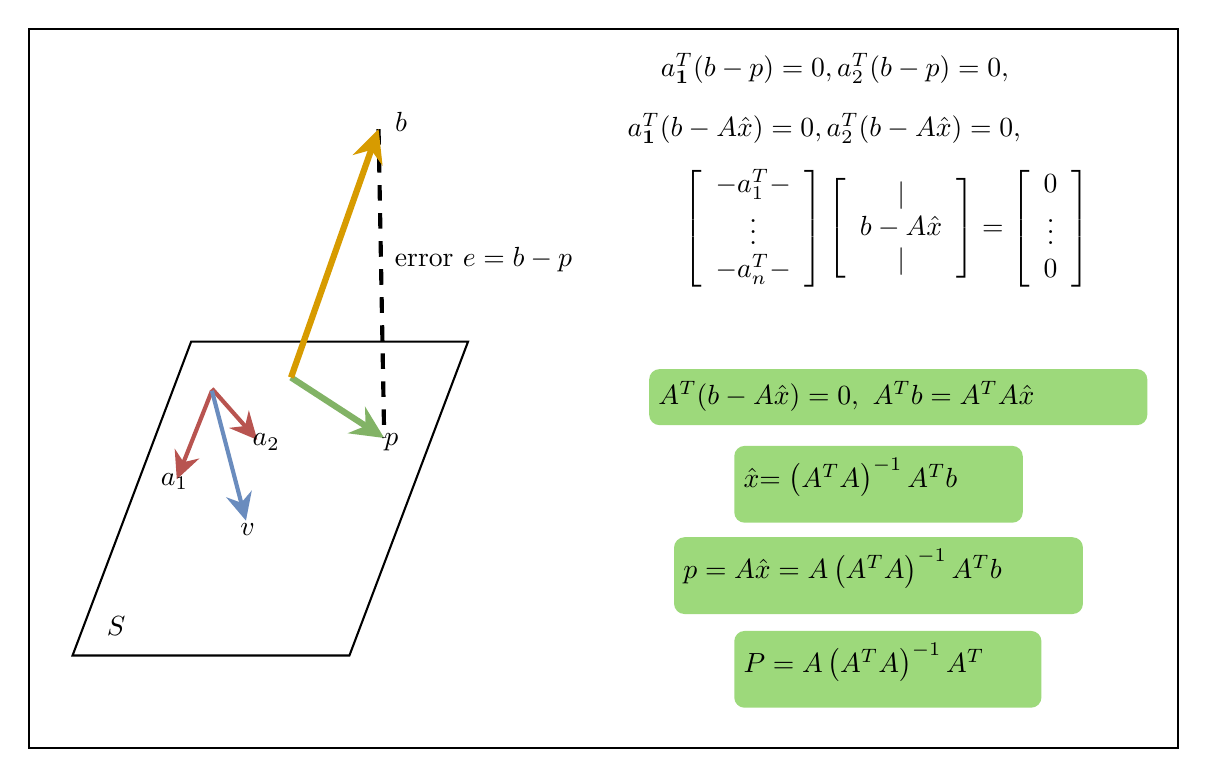
\begin{tikzpicture}[x=0.75pt,y=0.75pt,yscale=-1,xscale=1]
%uncomment if require: \path (0,350); %set diagram left start at 0, and has height of 350

%Straight Lines [id:da0833896477217686] 
\draw [color={rgb, 255:red, 130; green, 179; blue, 102 }  ,draw opacity=1 ][line width=2.25]    (127.38,169.03) -- (168.08,195.47) ;
\draw [shift={(172.28,198.19)}, rotate = 213] [fill={rgb, 255:red, 130; green, 179; blue, 102 }  ,fill opacity=1 ][line width=0.08]  [draw opacity=0] (16.07,-7.72) -- (0,0) -- (16.07,7.72) -- (10.67,0) -- cycle    ;
%Straight Lines [id:da7639150841734914] 
\draw [color={rgb, 255:red, 184; green, 84; blue, 80 }  ,draw opacity=1 ][line width=1.5]    (89.28,175.43) -- (73.82,214.38) ;
\draw [shift={(72.35,218.1)}, rotate = 291.64] [fill={rgb, 255:red, 184; green, 84; blue, 80 }  ,fill opacity=1 ][line width=0.08]  [draw opacity=0] (13.4,-6.43) -- (0,0) -- (13.4,6.44) -- (8.9,0) -- cycle    ;
%Straight Lines [id:da3617082286190523] 
\draw [line width=1.5]  [dash pattern={on 5.63pt off 4.5pt}]  (169.55,49.34) -- (172.28,198.19) ;
%Shape: Parallelogram [id:dp7592583426452624] 
\draw   (79.28,151.73) -- (212.68,151.73) -- (155.51,303) -- (22.11,303) -- cycle ;
%Straight Lines [id:da8449665178781662] 
\draw [color={rgb, 255:red, 184; green, 84; blue, 80 }  ,draw opacity=1 ][line width=1.5]    (89.28,174.43) -- (108.47,196.09) ;
\draw [shift={(111.12,199.08)}, rotate = 228.46] [fill={rgb, 255:red, 184; green, 84; blue, 80 }  ,fill opacity=1 ][line width=0.08]  [draw opacity=0] (13.4,-6.43) -- (0,0) -- (13.4,6.44) -- (8.9,0) -- cycle    ;
%Straight Lines [id:da21760172692551993] 
\draw [color={rgb, 255:red, 106; green, 140; blue, 190 }  ,draw opacity=1 ][line width=1.5]    (89.28,175.43) -- (104.64,234.14) ;
\draw [shift={(105.66,238.01)}, rotate = 255.32999999999998] [fill={rgb, 255:red, 106; green, 140; blue, 190 }  ,fill opacity=1 ][line width=0.08]  [draw opacity=0] (13.4,-6.43) -- (0,0) -- (13.4,6.44) -- (8.9,0) -- cycle    ;
%Straight Lines [id:da9743594112783229] 
\draw [color={rgb, 255:red, 215; green, 155; blue, 0 }  ,draw opacity=1 ][line width=2.25]    (127.38,169.03) -- (167.89,54.06) ;
\draw [shift={(169.55,49.34)}, rotate = 469.41] [fill={rgb, 255:red, 215; green, 155; blue, 0 }  ,fill opacity=1 ][line width=0.08]  [draw opacity=0] (16.07,-7.72) -- (0,0) -- (16.07,7.72) -- (10.67,0) -- cycle    ;
%Shape: Rectangle [id:dp3830905409317218] 
\draw   (1,1) -- (554.64,1) -- (554.64,347.62) -- (1,347.62) -- cycle ;

% Text Node
\draw (175.98,39.87) node [anchor=north west][inner sep=0.75pt]    {$\boldsymbol{b}$};
% Text Node
\draw (170.85,194.49) node [anchor=north west][inner sep=0.75pt]    {$\boldsymbol{p}$};
% Text Node
\draw (107.38,194.77) node [anchor=north west][inner sep=0.75pt]    {$\boldsymbol{a}_{2}$};
% Text Node
\draw (175.92,104.86) node [anchor=north west][inner sep=0.75pt]   [align=left] {error $\displaystyle \boldsymbol{e} =\boldsymbol{b-p}$};
% Text Node
\draw (63.21,213.92) node [anchor=north west][inner sep=0.75pt]    {$\boldsymbol{a}_{1}$};
% Text Node
\draw (101.48,237.88) node [anchor=north west][inner sep=0.75pt]    {$\boldsymbol{v}$};
% Text Node
\draw (37.18,282.9) node [anchor=north west][inner sep=0.75pt]    {$\boldsymbol{S}$};
% Text Node
\draw (288.11,40.4) node [anchor=north west][inner sep=0.75pt]    {$\boldsymbol{a}_{\mathbf{1}}^{T} (\boldsymbol{b} -\boldsymbol{A}\hat{\boldsymbol{x}} )=0,\boldsymbol{a}_{2}^{T} (\boldsymbol{b} -\boldsymbol{A}\hat{\boldsymbol{x}} )=0,\dotsc $};
% Text Node
\draw (304.11,11.4) node [anchor=north west][inner sep=0.75pt]    {$\boldsymbol{a}_{\mathbf{1}}^{T} (\boldsymbol{b} -\boldsymbol{p} )=0,\boldsymbol{a}_{2}^{T} (\boldsymbol{b} -\boldsymbol{p} )=0,\dotsc $};
% Text Node
\draw (314.93,67.4) node [anchor=north west][inner sep=0.75pt]    {$\left[\begin{array}{ c }
-\boldsymbol{a}_{1}^{{T}} -\\
\vdots \\
-\boldsymbol{a}_{n}^{{T}} -
\end{array}\right]\left[\begin{array}{ c }
\mid \\
\boldsymbol{b} -\boldsymbol{A\hat{\boldsymbol{x}}}\\
\mid 
\end{array}\right] =\left[\begin{array}{ c }
0\\
\vdots \\
0
\end{array}\right]$};
% Text Node
\draw  [color={rgb, 255:red, 0; green, 0; blue, 0 }  ,draw opacity=0 ][fill={rgb, 255:red, 157; green, 217; blue, 123 }  ,fill opacity=1 ]  (299.93,170) .. controls (299.93,167.24) and (302.17,165) .. (304.93,165) -- (534.93,165) .. controls (537.7,165) and (539.93,167.24) .. (539.93,170) -- (539.93,187) .. controls (539.93,189.76) and (537.7,192) .. (534.93,192) -- (304.93,192) .. controls (302.17,192) and (299.93,189.76) .. (299.93,187) -- cycle  ;
\draw (302.93,169.4) node [anchor=north west][inner sep=0.75pt]    {$\boldsymbol{A^{T} (b-A\hat{x} )} =0,\ \boldsymbol{A^{T} b=A^{T} A\hat{x}}$};
% Text Node
\draw  [color={rgb, 255:red, 0; green, 0; blue, 0 }  ,draw opacity=0 ][fill={rgb, 255:red, 157; green, 217; blue, 123 }  ,fill opacity=1 ]  (340.93,207) .. controls (340.93,204.24) and (343.17,202) .. (345.93,202) -- (474.93,202) .. controls (477.7,202) and (479.93,204.24) .. (479.93,207) -- (479.93,234) .. controls (479.93,236.76) and (477.7,239) .. (474.93,239) -- (345.93,239) .. controls (343.17,239) and (340.93,236.76) .. (340.93,234) -- cycle  ;
\draw (343.93,206.4) node [anchor=north west][inner sep=0.75pt]    {$\hat{\boldsymbol{x}}\boldsymbol{=\left( A^{T} A\right)^{-1} A^{T} b}$};
% Text Node
\draw  [color={rgb, 255:red, 157; green, 217; blue, 123 }  ,draw opacity=0 ][fill={rgb, 255:red, 157; green, 217; blue, 123 }  ,fill opacity=1 ]  (311.93,251) .. controls (311.93,248.24) and (314.17,246) .. (316.93,246) -- (503.93,246) .. controls (506.7,246) and (508.93,248.24) .. (508.93,251) -- (508.93,278) .. controls (508.93,280.76) and (506.7,283) .. (503.93,283) -- (316.93,283) .. controls (314.17,283) and (311.93,280.76) .. (311.93,278) -- cycle  ;
\draw (314.93,250.4) node [anchor=north west][inner sep=0.75pt]    {$\boldsymbol{p=A\hat{x} =A\left( A^{T} A\right)^{-1} A^{T} b}$};
% Text Node
\draw  [color={rgb, 255:red, 0; green, 0; blue, 0 }  ,draw opacity=0 ][fill={rgb, 255:red, 157; green, 217; blue, 123 }  ,fill opacity=1 ]  (340.93,296.15) .. controls (340.93,293.38) and (343.17,291.15) .. (345.93,291.15) -- (483.93,291.15) .. controls (486.7,291.15) and (488.93,293.38) .. (488.93,296.15) -- (488.93,323.15) .. controls (488.93,325.91) and (486.7,328.15) .. (483.93,328.15) -- (345.93,328.15) .. controls (343.17,328.15) and (340.93,325.91) .. (340.93,323.15) -- cycle  ;
\draw (343.93,295.55) node [anchor=north west][inner sep=0.75pt]    {$\boldsymbol{P=A\left( A^{T} A\right)^{-1} A^{T}}$};


\end{tikzpicture}

\end{FigureCenter}

\begin{FigureCenter}{Projecting onto the column space of $A$ is also projecting onto the column space of $Q$}
    \tikzset{every picture/.style={line width=0.75pt}} %set default line width to 0.75pt

\begin{tikzpicture}[x=0.75pt,y=0.75pt,yscale=-1,xscale=1]
%uncomment if require: \path (0,300); %set diagram left start at 0, and has height of 300

%Shape: Parallelogram [id:dp16734778977883136] 
\draw  [color={rgb, 255:red, 255; green, 255; blue, 255 }  ,draw opacity=1 ][fill={rgb, 255:red, 179; green, 179; blue, 179 }  ,fill opacity=1 ] (224.15,98.88) -- (563.14,98.88) -- (417.85,242.95) -- (78.86,242.95) -- cycle ;
%Straight Lines [id:da3519715103345966] 
\draw [color={rgb, 255:red, 0; green, 0; blue, 0 }  ,draw opacity=1 ][line width=1.5]  [dash pattern={on 1.69pt off 2.76pt}]  (399.96,59.43) -- (399.07,151.88) ;
%Straight Lines [id:da7143500773565701] 
\draw [color={rgb, 255:red, 74; green, 144; blue, 226 }  ,draw opacity=1 ][line width=2.25]    (252.07,166.88) -- (395.92,62.37) ;
\draw [shift={(399.96,59.43)}, rotate = 504] [fill={rgb, 255:red, 74; green, 144; blue, 226 }  ,fill opacity=1 ][line width=0.08]  [draw opacity=0] (14.29,-6.86) -- (0,0) -- (14.29,6.86) -- cycle    ;
%Straight Lines [id:da29623635442698415] 
\draw [color={rgb, 255:red, 234; green, 81; blue, 100 }  ,draw opacity=1 ][line width=2.25]    (252.07,166.88) -- (394.09,152.39) ;
\draw [shift={(399.07,151.88)}, rotate = 534.1700000000001] [fill={rgb, 255:red, 234; green, 81; blue, 100 }  ,fill opacity=1 ][line width=0.08]  [draw opacity=0] (14.29,-6.86) -- (0,0) -- (14.29,6.86) -- cycle    ;

% Text Node
\draw (114.72,185.99) node [anchor=north west][inner sep=0.75pt]    {$\begin{aligned}
C( A) & =C( Q)\\
\operatorname{range}( A) & =\operatorname{range}( Q)
\end{aligned}$};
% Text Node
\draw (376.21,43.4) node [anchor=north west][inner sep=0.75pt]    {$x$};
% Text Node
\draw  [color={rgb, 255:red, 0; green, 0; blue, 0 }  ,draw opacity=0 ][fill={rgb, 255:red, 234; green, 81; blue, 100 }  ,fill opacity=1 ]  (347.57,167.38) .. controls (347.57,164.62) and (349.8,162.38) .. (352.57,162.38) -- (463.57,162.38) .. controls (466.33,162.38) and (468.57,164.62) .. (468.57,167.38) -- (468.57,182.38) .. controls (468.57,185.14) and (466.33,187.38) .. (463.57,187.38) -- (352.57,187.38) .. controls (349.8,187.38) and (347.57,185.14) .. (347.57,182.38) -- cycle  ;
\draw (350.57,166.78) node [anchor=north west][inner sep=0.75pt]    {$AA^{\dagger } x=QQ^{T} x$};


\end{tikzpicture}
\end{FigureCenter}

矩阵 $ {A} \in \mathbb{R}^{m \times n} $ 的列 $ a_{1}, a_{2}, \ldots, a_{n} \in \mathbb{R}^{m} $ 的最小二乘法问题
\begin{equation}
\hat{x}=\underset{x}{\arg \underset{x}{\min}}\|A x-b\|_{2}^{2} ,\|A x-b\|_{2}^{2}=\left\|\sum_{j=1}^{n} a_{j} x_{j}-b\right\|_{2}^{2}
\end{equation}

向量 $ b $ 在 $ \operatorname{range}(A) $ 上的投影是 $ A\left(A^{T} A\right)^{-1} A^{T} b $.

残差向量 $ \hat{r}=A \hat{x}-b $ 满足 $ A^{T} \hat{r}=A^{T}(A \hat{x}-b)=0 $.残差向量 $ \hat{r} $ 正交于 $ A $ 的每一列,因此正交于$ \operatorname{range}(A) $.




\begin{theorem}[投影与$A$列空间的关系]
    $ A \hat{x} \in \operatorname{range}(A) $是$A$的列空间中最接近$b$的向量。 
    
    $ \hat{r}=A \hat{x} -b$正交于$A$的列空间(值域空间) $ \operatorname{range}(A) $.
\end{theorem}

\section{正规方程}

\begin{theorem}[最小二乘法问题的正规方程]

    \begin{equation} \nabla f(x)=0, f(x)=\|A x-b\|_{2}^{2} \end{equation}
等价于
\begin{equation}
A^{T} A x=A^{T} b
\end{equation}
\end{theorem}

系数矩阵 $ A^{T} A $ 是 $ A $ 的Gram矩阵,最小二乘法问题所有的解都满足正规方程。

\begin{theorem}
    如果A的列线性无关,则

    $ A^{T} A $ 为非奇异矩阵,正规方程此时有唯一解。
\end{theorem}


\section{QR分解求解最小二乘法}

\begin{theorem}[QR分解求解最小二乘法]
    若 $ {A} \in \mathbb{R}^{m \times n} $ 的列向量线性无关,则存在 $ {A}={QR} $ 分解, $ Q \in \mathbb{R}^{m \times n} $ , $ R \in \mathbb{R}^{{n} \times n} $ 
    
    最小二乘法问题的解
\begin{equation}
\begin{aligned}
\hat{x}&=\left(A^{T} A\right)^{-1} A^{T} b \\
&=\left((Q R)^{T}(Q R)\right)^{-1}(Q R)^{T} b \\
&=\left(R^{T} Q^{T} Q R\right)^{-1} R^{T} Q^{T} b \\
&=\left(R^{T} R\right)^{-1} R^{T} Q^{T} b \\
&=R^{-1} Q^{T} b
\end{aligned}
\end{equation}
\end{theorem}


\begin{example}
    \begin{equation}
A=\left[\begin{array}{cc}
3 & -6 \\
4 & -8 \\
0 & 1
\end{array}\right], \quad b=\left[\begin{array}{c}
-1 \\
7 \\
0
\end{array}\right]
\end{equation}
首先对$A$进行QR分解
\begin{equation}
Q=\left[\begin{array}{cc}
3 / 5 & 0 \\
4 / 5 & 0 \\
0 & 1
\end{array}\right], \quad R=\left[\begin{array}{cc}
5 & -10 \\
0 & 1
\end{array}\right]
\end{equation}

计算 $ d=Q^{T} b=(5,2) $

求解 $ R x=d $
\begin{equation}
\left[\begin{array}{cc}
5 & -10 \\
0 & 1
\end{array}\right]\left[\begin{array}{l}
x_{1} \\
x_{2}
\end{array}\right]=\left[\begin{array}{l}
5 \\
2
\end{array}\right]
\end{equation}

解得 $ x_{1}=5, x_{2}=2 $

\end{example}


\subsection{The Complexity of Solving Least Square Problem via QR Decomposition}

算法复杂度:

\begin{itemize}
    \item 首先对A进行QR分解 $ A=Q R\left(2 m n^{2}\right. $ flops $ ) $
    \item 计算矩阵向量乘积 $ d=Q^{T} b(2 {mn} $ flops $ ) $
    \item 通过回代求解 $ R x=d\left(n^{2}\right. $ flops $ ) $
    \item 复杂度: $ 2 m n^{2} $ flops
\end{itemize}



\section{求解正规方程可能带来的严重误差}

直接求解正规方程组求解:
\begin{equation}
A^{T} A x=A^{T} b
\end{equation}

可能会造成严重的舍入误差。

\begin{example}
    一个列向量“几乎”线性相关的矩阵
\begin{equation}
A=\left[\begin{array}{cc}
1 & -1 \\
0 & 10^{-5} \\
0 & 0
\end{array}\right],  b=\left[\begin{array}{c}
0 \\
10^{-5} \\
1
\end{array}\right]
\end{equation}

将中间结果四舍五入到小数点后8位。

方法 1 :通过Gram矩阵求解
\begin{equation}
A^{T} A=\left[\begin{array}{cc}
1 & -1 \\
-1 & 1+10^{-10}
\end{array}\right] \approx\left[\begin{array}{cc}
1 & -1 \\
-1 & 1
\end{array}\right], A^{T} b=\left[\begin{array}{c}
0 \\
10^{-10}
\end{array}\right] \Rightarrow x=\left[\begin{array}{c}
10^{-10} \\
10^{-10}
\end{array}\right]
\end{equation}
经过四舍五入之后,Gram矩阵为奇异矩阵。


方法 2 : 通过对 $A$进行QR分解
\begin{equation}
Q=\left[\begin{array}{ll}
1 & 0 \\
0 & 1 \\
0 & 0
\end{array}\right],  R=\left[\begin{array}{cc}
1 & -1 \\
0 & 10^{-5}
\end{array}\right]
\end{equation}

\begin{equation}\begin{aligned}
    &\hat{x}=\left(A^{T} A\right)^{-1} A^{T} b=R^{-1} Q^{T} b \\
    \Rightarrow& R x=Q^{T} b\\
    \Rightarrow& \left[\begin{array}{cc}1 & -1 \\ 0 & 10^{-5}\end{array}\right]\left[\begin{array}{l}x_{1} \\ x_{2}\end{array}\right]=\left[\begin{array}{l}0 \\ 10^{-5}\end{array}\right] \\
    \Rightarrow& x=\left[\begin{array}{l}1 \\ 1\end{array}\right]
\end{aligned}\end{equation}

\end{example}

方法2 比方法1更稳定,因为它避免构造Gram矩阵。



\section{梯度下降法}

给定 $ A \in \mathbb{R}^{m \times n}, {~b} \in \mathbb{R}^{m}, x \in \mathbb{R}^{n} $ 目标函数:
\begin{equation}
f(x)=\|A x-b\|_{2}^{2}=\sum_{i=1}^{m}\left(\sum_{j=1}^{n} A_{i j} x_{j}-b_{i}\right)^{2}
\end{equation}
为使目标函数最小, 可求最优解 $ \hat{x}: \quad \hat{x}=\arg \underset{x}{ \min } f(x) $.

\begin{problem}
    $ A \in \mathbb{R}^{{m} \times n} $ 列向量线性相关或n非常大$
    A^{T} A \in \mathbb{R}^{n \times n}$不可逆,无法直接代入求得最小二乘解。
\end{problem}

通过迭代求解目标的最优解过程: \begin{equation} x^{(1)}, x^{(2)}, \cdots, x^{(k)} \rightarrow \hat{x} \end{equation} 

设 $ x^{(k)} $ 是第$k$步迭代,期望更新 $ x^{(k+1)} $ ,满足 $ f\left(x^{(k+1)}\right)<f\left(x^{(k)}\right) $.

设函数 $ f(x) $ 可微,根据泰勒公式,在 $ x^{(k)} $ 的一阶公式为
\begin{equation}
f\left(x^{(k+1)}\right)=f\left(x^{(k)}\right)+\left\langle\nabla f\left(x^{(k)}\right), x^{(k+1)}-x^{(k)}\right\rangle+o\left(\left\|x^{(k+1)}-x^{(k)}\right\|\right)
\end{equation}

如果 $ \left\|x^{(k+1)}-x^{(k)}\right\|_{2} $ 足够小, 则有
\begin{equation}
f\left(x^{(k+1)}\right)-f\left(x^{(k)}\right) \approx\left\langle\nabla f\left(x^{(k)}\right), x^{(k+1)}-x^{(k)}\right\rangle
\end{equation}

\begin{corollary}
    根据Cauchy-Schwarz不等式 \ref{thm:cauchy-schwartz=inequality}

    $ \left|\left\langle\nabla f\left(x^{(k)}\right), x^{(k+1)}-x^{(k)}\right\rangle\right| \leq\left\|\nabla f\left(x^{(k)}\right)\right\|_{2}\left\|x^{(k+1)}-x^{(k)}\right\|_{2} $

    所以有
    \begin{equation}
\left\langle\nabla f\left(x^{(k)}\right), x^{(k+1)}-x^{(k)}\right\rangle \geq -\left\|\nabla f\left(x^{(k)}\right)\right\|_{2}\left\|x^{(k+1)}-x^{(k)}\right\|_{2}
\end{equation}

当 $ x^{(k+1)}-x^{(k)}=-\alpha_{k} \nabla f\left(x^{(k)}\right), \alpha_{k}>0 $ 时,等式成立。

由于$-\left\|\nabla f\left(x^{(k)}\right)\right\|_{2}\left\|x^{(k+1)}-x^{(k)}\right\|_{2}$是非负的,此时$f\left(x^{(k+1)}\right)-f\left(x^{(k)}\right) \le 0$.
\end{corollary}

迭代公式为 

\begin{equation}  x^{(k+1)}=x^{(k)}-\alpha_{k} \nabla f\left(x^{(k)}\right) , f\left(x^{(k+1)}\right)<f\left(x^{(k)}\right) \end{equation}


\begin{definition}[梯度下降法求解最小二乘法]
    \begin{equation}
\min _{x \in \mathbb{R}^{n}} \frac{1}{2}\|A x-b\|_{2}^{2}, \quad A \in \mathbb{R}^{m \times n}, b \in \mathbb{R}^{m}
\end{equation}

令 \begin{equation} f(x)=\frac{1}{2}\|A x-b\|_{2}^{2} \end{equation}

则 $ f $ 为凸函数, 并有 $ \nabla f(x)=A^{T}(A x-b) $.

则 $ A^{T} A \in \mathbb{R}^{n \times n} $ .如果列向量\textbf{线性相关}会导致其\textbf{不可逆}或$n$非常大。可以通过梯度下降法迭代

\begin{equation}  x^{(k+1)}=x^{(k)}-\alpha_{k} \nabla f\left(x^{(k)}\right) , f\left(x^{(k+1)}\right)<f\left(x^{(k)}\right) \end{equation}

求解

\begin{equation} x^{(k+1)}=x^{(k)}-\alpha^{(k)} A^{T}\left(A x^{(k)}-b\right) \end{equation}
\end{definition}


\begin{algorithm}[htbp]
    \caption{梯度下降法}
    初始化 $ x^{(0)} $, $k=0$\;
    \While(){Not Convergent}{
        $p^{(k)}=A^{T}\left(A x^{(k)}-b\right)$\;
        $x^{(k+1)}=x^{(k)}-\alpha^{(k)} p^{(k)}$\;
        $k \leftarrow k + 1$
    }
\end{algorithm}

\section{估计学习率(步长)$\alpha$}

\begin{problem}
    \begin{equation}
    \min _{x \in \mathbb{R}^{n}} \frac{1}{2}\|A x-b\|_{2}^{2}, \quad A \in \mathbb{R}^{m \times n}, b \in \mathbb{R}^{m}
    \end{equation}
    
    令 $ f(x)=\frac{1}{2}\|A x-b\|_{2}^{2} $

    \begin{equation} x^{(k+1)}=x^{(k)}-\alpha^{(k)} A^{T}\left(A x^{(k)}-b\right) \end{equation}

    需要估计 $ \alpha^{(k)} $.
\end{problem}

为了估计 $ \alpha^{(k)} $, 通过线性搜索估计:
\begin{equation}
\alpha^{(k)}=\arg \min _{\alpha \in \Re} f\left(x^{(k)}-\alpha A^{T}\left(A x^{(k)}-b\right)\right)
\end{equation}

即 $ \alpha^{(k)} $ 是最优步长。在上面的优化式中$x^{(k)}$、$A$、$b$均视为定值。

\begin{theorem}[线性搜索估计的最优步长]
    \begin{equation}\alpha^{(k)}=\frac{\left\|A^{T}\left(A x^{(k)}-b\right)\right\|_{2}^{2}}{\left\|A A^{T}\left(A x^{(k)}-b\right)\right\|_{2}^{2}}\end{equation}
\end{theorem}

\begin{proof}
    令 $ g(\alpha)=f\left(x^{(k)}-\alpha A^{T}\left(A x^{(k)}-b\right)\right) $ 是关于 $ \alpha $ 的 凸函数, 则有

\begin{equation}
\min _{\alpha} g(\alpha) \Rightarrow g^{\prime}(\alpha)=0 \Rightarrow \alpha^{(k)}=\frac{\left\|A^{T}\left(A x^{(k)}-b\right)\right\|_{2}^{2}}{\left\|A A^{T}\left(A x^{(k)}-b\right)\right\|_{2}^{2}}
\end{equation}


\begin{equation}\begin{aligned}
    & f(x)=\frac{1}{2}\|A x-b\|_{2}^{2}, g\left(\alpha^{(k)}\right)=f\left({\color{violet} x^{(k)}-\alpha^{(k)} A^{T}\left(A x^{(k)}-b\right)} \right) \\
    \Rightarrow & g\left(\alpha^{(k)}\right)=\frac{1}{2}\left\|A\left({\color{violet} x^{(k)}-\alpha^{(k)} A^{T}\left(A x^{(k)}-b\right)} \right)-b\right\|_{2}^{2} \\
    &=\frac{1}{2}\left\|\left({\color{coral} A x^{(k)}-b} \right)-\left({\color{grass} \alpha^{(k)} A^{T}\left(A x^{(k)}-b\right)} \right)\right\|_{2}^{2} \\
    &=\frac{1}{2}\left(\left({\color{coral} A x^{(k)}-b} \right)^{T}\left({\color{coral} A x^{(k)}-b} \right)+\left({\color{grass} \alpha^{(k)} A^{T}\left(A x^{(k)}-b\right)} \right)^{T}\left({\color{grass} \alpha^{(k)} A^{T}\left(A x^{(k)}-b\right)} \right)\right) \\
    &-\left({\color{coral} A x^{(k)}-b} \right)^{T}\left({\color{grass} \alpha^{(k)} A^{T}\left(A x^{(k)}-b\right)} \right) \\
    \Rightarrow & g^{\prime}\left(\alpha^{(k)}\right)=\alpha^{(k)}\left(A^{T}\left(A x^{(k)}-b\right)\right)^{T}\left(A^{T}\left(A x^{(k)}-b\right)\right)-\left(A x^{(k)}-b\right)^{T}\left(A^{T}\left(A x^{(k)}-b\right)\right)=0 \\
    \Rightarrow &\alpha^{(k)}=\frac{\left\|A^{T}\left(A x^{(k)}-b\right)\right\|_{2}^{2}}{\left\|A A^{T}\left(A x^{(k)}-b\right)\right\|_{2}^{2}}
    \end{aligned}\end{equation}

\end{proof}


\begin{algorithm}[htbp]
    \caption{使用线性搜索估计步长的梯度下降法}
    初始化 $ x^{(0)} $, $k=0$\;
    \While(){Not Convergent}{
        $p^{(k)}=A^{T}\left(A x^{(k)}-b\right)$\;
        $\alpha^{(k)}=\dfrac{\left\|p^{(k)}\right\|_{2}^{2}}{\left\|A p^{(k)}\right\|_{2}^{2}}$\;
        $x^{(k+1)}=x^{(k)}-\alpha^{(k)} p^{(k)}$\;
    }
\end{algorithm}